\documentclass{article}
\usepackage{graphicx}
\usepackage{enumitem}
\begin{document}
\title{physics}
\author{Pawan Kalyan}
\maketitle
\begin{enumerate}
	\item Which one of the following options is CORRECT for the given circuit ?
		\begin{figure}[h]
			\centering
			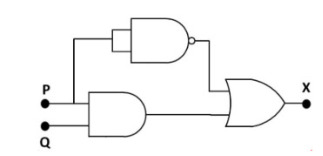
\includegraphics[width=\columnwidth]{FIG/Q24.jpg}
		\end{figure}

		\begin{enumerate}[label=(\Alph*)]
		\item P = $1$, Q = $1$ ; X = $0$
		\item P = $1$, Q = $0$ ; X = $1$
		\item P = $0$, Q = $1$ ; X = $0$
		\item P = $0$, Q = $0$ ; X = $1$
	\end{enumerate}
\end{enumerate}
\end{document}


